\documentclass[11pt,reqno]{amsart}
\usepackage[top=1in, left=1in, right=1in, bottom=1in]{geometry}                % See geometry.pdf to learn the layout options. There are lots.
\geometry{letterpaper}                   % ... or a4paper or a5paper or ... 
\usepackage[parfill]{parskip}    % Activate to begin paragraphs with an empty line rather than an indent
%\usepackage{algorithm, algorithmic}

\usepackage{algorithm}
\usepackage{algpseudocode}

\usepackage{graphicx}

\usepackage{verbatim}
\usepackage{amssymb}
\usepackage{amsmath}

\usepackage{enumitem}

\usepackage{setspace}
\doublespacing

\usepackage{natbib}

%\usepackage{epstopdf}
%\DeclareGraphicsRule{.tif}{png}{.png}{`convert #1 `dirname #1`/`basename #1 .tif`.png}

\newcommand{\RR}{I\!\!R} %real numbers
\DeclareMathOperator{\diag}{diag}

\algnewcommand{\Inputs}[1]{%
  \State \textbf{Inputs:}
  \Statex \hspace*{\algorithmicindent}\parbox[t]{.8\linewidth}{\raggedright #1}
}
\algnewcommand{\Initialize}[1]{%
  \State \textbf{Initialize:}
  \Statex \hspace*{\algorithmicindent}\parbox[t]{.8\linewidth}{\raggedright #1}
}

\title[RVD2]{RVD2: An ultra-sensitive variant detection model for low-depth targeted next-generation sequencing data}
\author{}
%\date{}                                           % Activate to display a given date or no date

\begin{document}

\begin{abstract}
Next-generation sequencing technology is increasingly being used for clinical diagnostic tests. Clinical samples are often genomically heterogeneous due to low sample purity or the presence of genetic subpopulations. However, many variant calling algorithms are optimized to call single nucleotide polymorphisms in homogeneous rather than heterogeneous samples. We present a novel variant calling algorithm that uses a hierarchical Bayesian model to estimate allele frequency and call variants in heterogeneous samples. We show that our algorithm improves upon current classifiers and has higher sensitivity and specificity over wide ranges of median read depth and a minor allele frequency. We identify five mutations in the PAXP1 gene in a matched clinical breast ductal carcinoma tumor sample; two of which are loss-of-heterozygosity events.

%Unmasked positions has median read depth 51 for control sample, and 69 for case sample (from folder '2013-11-22_HCC1187_PAXIP1_genome_Qsd_0_1'; masked positions has median read depth 52 for control sample, and 70 for case sample( from foler '2013-11-22_HCC1187_PAXIP1_hg19masked_Qsd_0_1')
%We use our algorithm to call variants in a pooled sample of 100 patients with multiple sclerosis and identify novel variants in IL7RA and IL2R.
\end{abstract}

\maketitle

\section{Introduction}

Next-generation sequencing (NGS) technology has enabled the systematic interrogation of the genome for a fraction of the cost of traditional assays~\citep{Koboldt:2013kw}. Protocol and platform engineering improvements have enabled the generation of $1\times10^9$ bases of sequence data in 27 hours for approximately \$1000~\citep{Quail:2012hf}. As a result, NGS is increasingly being used as a general platform for research assays for methylation state~\citep{Laird:2010ab}, DNA mutations~\citep{Consortium:2013co}, copy number variation~\citep{Alkan:2009cr}, promoter occupancy~\citep{Ouyang:2009hc} and others~\citep{Rivera:2013ee}. NGS diagnostics are being translated to clinical applications including noninvasive fetal diagnostics~\citep{Kitzman:2012hea}, infectious disease diagnostics~\citep{Capobianchi:2012em}, cancer diagnostics~\citep{Navin:2010gu}, and human microbial analysis~\citep{Consortium:2013iz}. 

Increasingly, NGS is being used to interrogate mutations in heterogeneous clinical samples. For example, NGS-based non-invasive fetal DNA testing uses maternal blood sample to sequence the minority fraction of cell-free fetal DNA~\citep{Fan:2008di}. Infectious diseases such as HIV and influenza may contain many genetically heterogeneous sub-populations~\citep{Flaherty:2011ja, Ghedin:2010ie}. DNA sequencing of individual regions of a solid tumor has revealed genetic heterogeneous within an individual sample~\citep{Navin:2010gu}.  

However, the primary statistical tools for calling variants from NGS data are optimized for homogeneous samples. Most analysis pipelines make use of preprocessing or postprocessing or both to eliminate error prone reads and false positives. Samtools/bcftools and GATK a naive Bayes decision rule to call a variant~\citep{}. GATK involves more sophisticate pre and post-processing steps. The genotype prior is fixed and constant across all loci and the likelihood of an allele at a locus is a function of the phred score~\citep{McKenna:2010bv}.

Recently, researchers have developed algorithms to call low-frequency or rare variants in heterogeneous samples.  VarScan2 combines algorithmic heuristics to call genotypes in the tumor and normal sample pileup data and then applies a Fisher's exact test on the read count data to detect a significant difference in the genotype calls~\citep{Koboldt:2012cg}. Strelka uses a hierarchical Bayesian approach to model the joint distribution of the allele frequency in the tumor and normal samples at each locus~\citep{Saunders:2012fh}. With the joint distribution available, one is able to identify locations with dissimilar allele frequencies. muTect uses a Bayesian posterior probability in its decision rule to evaluate the likelihood of a mutation~\citep{Cibulskis:2013ta}.

Typically such a variant calling algorithms are comprised of multiple pre- and post-filtration steps around model estimation and hypothesis testing steps~\citep{Pabinger:2013dl}. These steps may improve algorithm performance, but their presence makes it difficult to isolate what step is most responsible for the performance. Instead, we focus exclusively on the model structure and statistical inference steps. Additional filtration steps may improve performance considerably, but those aspects are subjects of intense research and separate study. We have isolated the statistical inference and hypothesis testing steps so that they may be used independently or as part of a larger variant calling pipeline.

We present the hierarchical Bayesian model in Section~\ref{sec:model_structure} and a Bayesian hypothesis test to detect mutations in Section~\ref{sec:hypothesis_test}. In Section~\ref{sec:read_depth} we present sensitivity and specificity results of our method on known, pure DNA samples mixed at defined fractions. We compare our algorithm to the most accurate methods available to date in Section~\ref{sec:comparison}. Finally, in Section~\ref{sec:brca} we present results on detecting mutations in the PAXIP1 gene from matched tumor-normal data from the HCC1187 cell line.

%%%%%%%%%%%%%%%%%%
% Model Structure
%%%%%%%%%%%%%%%%%%
\section{Model Structure}\label{sec:model_structure}


RVD uses a two-stage approach for detecting for rare variants. First, it estimates the parameters of two hierarchical Bayesian models; one using data from the sample of interest (case) and one using data from a known reference sample (control). Then, it tests for a significant difference between model parameters in the case and control samples and returns called variant positions.

For a given sample, the observed data consists of two matrices $r \in \RR^{J \times N}$ and $n \in \RR^{J \times N}$, where $r_{ji}$ is the number of reads with a non-reference base at location $j$ in experimental replicate $i$ and $n_{ji}$ is the total number of reads at location $j$ in replicate $i$. The generative process is as follows:

\begin{enumerate}[noitemsep]
	\item For each location $j$: 
	\begin{enumerate}
		\item Draw an error rate $\mu_j \thicksim \text{Beta}(\mu_0, M_0)$
		\item For each replicate $i$:
		\begin{enumerate}
			\item Draw $\theta_{ji} \thicksim \text{Beta}(\mu_j, M_j)$
			\item Draw $r_{ji} | n_{ji} \thicksim \text{Binomial}(\theta_{ji}, n_{ji})$
		\end{enumerate}
	\end{enumerate}
\end{enumerate}

This process involves several hyperparameters: $\mu_0$, a global error rate; $M_0$, a global precision; $M_j$, a local precision. The global error rate, $\mu_0$, estimates the expected error rate across all locations. The global precision, $M_0$, estimates the variation in the error rate  across locations. The local precision, $M_j$, estimates the variation in the error rate across replicates at location $j$.

RVD2 has three levels of sampling. First, a global error rate and global precision are chosen once for the entire data set. Then, at each location, a local precision is chosen and a local error rate is sampled from a Beta distribution. Finally, the error rate for replicate $i$ at location $j$ is drawn from a Beta distribution and the number of non-reference reads is drawn from a binomial.

RVD2 hierarchically partitions sources of variation in the data. $r_{ji} | n_{ji} \thicksim \text{Binomial}(\theta_{ji}, n_{ji})$ models the variation due to sampling the pool of DNA molecules on the sequencer. $\theta_{ji} \thicksim \text{Beta}(\mu_j, M_j)$ models the variation due to experimental reproducibility. The variation in error rate due to sequence context is modeled by $\mu_j \thicksim \text{Beta}(\mu_0, M_0)$. Importantly, increasing the read depth $n_{ji}$ only reduces the sampling error, but does nothing to reduce experimental variation or variation due to sequence context.

\begin{figure}[h]
\begin{center}
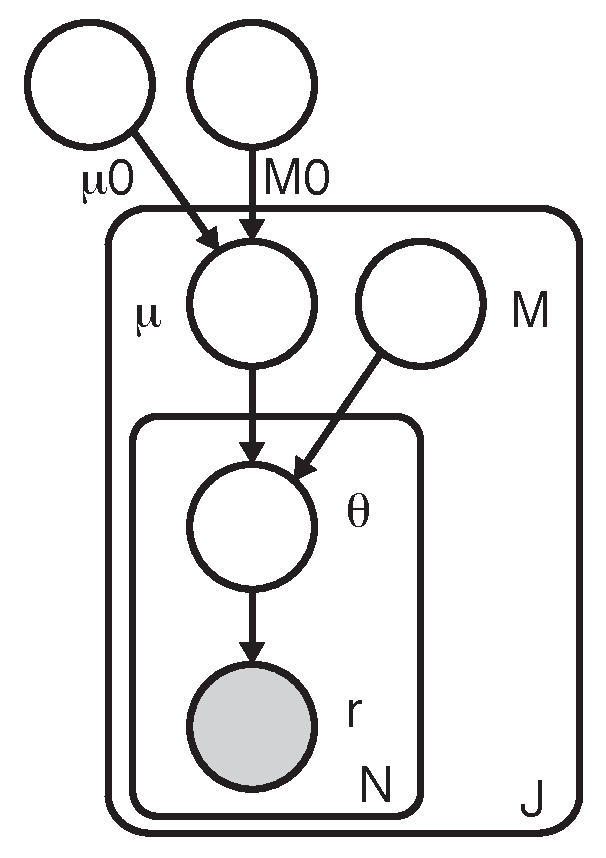
\includegraphics[width=40mm]{pdf_figs/RVD2_model.pdf}
\caption{RVD2 Graphical Model}
\label{fig:graphical_model}
\end{center}
\end{figure}

Figure~\ref{fig:graphical_model} shows a graphical representation of the RVD2 statistical model. In this graphical model framework a shaded node represents an observed random variable, an unshaded node represents an unobserved or latent random variable and a directed edge represents a functional dependency between the two connected nodes~\cite{}. A rounded box or ``plate" represents replication of the nodes within the plate. This graphical model framework connects graph theory and probability theory in a way that facilitates algorithmic methods for statistical inference.

The joint distribution over the latent and observed variables for data at location $j$ in replicate $i$ given the parameters is

\begin{equation}\label{eqn:jointpdf}
p \left( r_{ji}, \theta_{ji}, \mu_j | n_{ji}; \mu_0, M_0, M_j \right) = p \left( r_{ji} | \theta_{ji}, n_{ji} \right) p\left( \theta_{ji} | \mu_j; M_j \right) p\left( \mu_j; \mu_0, M_0 \right)
\end{equation}

The individual conditional distributions are:
\begin{align}
p\left( \mu_j; \mu_0, M_0 \right)  &= \frac{ \Gamma(M_0) } { \Gamma(\mu_0 M_0) \Gamma(M_0 (1-\mu_0)) } \mu_j^{M_0\mu_0 -1} (1 - \mu_j)^{M_0 ( 1 - \mu_0) - 1}, \nonumber \\
p\left( \theta_{ji} | \mu_j; M_j \right) &= \frac{ \Gamma(M_j) } { \Gamma(\mu_j M_j) \Gamma(M_j (1-\mu_j)) } \theta_{ji}^{M_j\mu_j -1} (1 - \theta_{ji})^{M_j ( 1 - \mu_j) - 1}, \nonumber \\
p \left( r_{ji} | \theta_{ji}, n_{ji} \right) &= \frac{ \Gamma(n_{ji}+1) } { \Gamma(r_{ji}+1) \Gamma( n_{ji} - r_{ji} + 1 ) } \theta_{ji}^{r_{ji}} (1 - \theta_{ji})^{n_{ji} - r_{ji}}. \nonumber
\end{align}

Integrating over the latent variables $\theta_{ji}$ and $\mu_j$ yields the marginal distribution of the data at location $j$ in replicate $i$, 
\begin{equation}
p \left( r_{ji} | n_{ji} ; \mu_0, M_0, M_j \right) = \int_{\mu_j} \int_{\theta_{ji}}  p \left( r_{ji} | \theta_{ji}, n_{ji} \right) p\left( \theta_{ji} | \mu_j; M_j \right) p\left( \mu_j; \mu_0, M_0 \right) d\theta_{ji} d\mu_j.
\end{equation}

Finally, the complete log-likelihood for the data set is

\begin{equation}
\log p \left( r | n ; \mu_0, M_0, M \right) = \sum_{j=1}^J \sum_{i=1}^N \log \int_{\mu_j} \int_{\theta_{ji}}  p \left( r_{ji} | \theta_{ji}, n_{ji} \right) p\left( \theta_{ji} | \mu_j; M_j \right) p\left( \mu_j; \mu_0, M_0 \right) d\theta_{ji} d\mu_j.
\end{equation}


%%%%%%%%%%%%%%%%%%
% Inference & Hypothesis Testing
%%%%%%%%%%%%%%%%%%
\section{Inference and Hypothesis Testing}

The primary object of inference in this model is the joint posterior distribution function over the latent variables,
\begin{equation}
	p(\mu, \theta | r, n; \phi)  = \frac{ p(\mu, \theta, r | n; \phi) } {p ( r | n; \phi)},
\end{equation}
where the parameters are $\phi \triangleq \{\mu_0, M_0, M\}$.

The Beta distribution over $\mu_j$ is conjugate to the Binomial distribution over $\theta_{ji}$, so we can write the posterior distribution as a Beta distribution. However, there is not a closed form for the product of a Beta distribution with another Beta distribution and exact inference is intractable.  exact inference is intractable.

Instead, we have developed a Metropolis-within-Gibbs  approximate inference algorithm shown in Algorithm~\ref{alg:metro_gibbs}. First, the hyperparameters are initialized using method-of-moments (MoM). Given those hyperparameter estimates, we sample from the marginal posterior distribution for $\mu_j$ given its Markov blanket using a Metropolis-Hasting rejection sampling rule. Finally, we sample from the marginal posterior distribution for $\theta_{ji}$ given its Markov blanket. Samples from $\theta_{ji}$ can be drawn from the posterior distribution directly  because the prior and likelihood form a conjugate pair. This sampling procedure is repeated until the chain converges to a stationary distribution then we draw samples from the posterior distribution over latent variables.

\begin{algorithm}[ht]
\caption{Metropolis-within-Gibbs Algorithm}
\label{alg:metro_gibbs}
\begin{algorithmic}[1]

\State Initialize $\theta$, $\mu$, $M$, $\mu_0$, $M_0$
\Repeat
\For {each location j} \Comment{Sample $\mu_j$}
  \State Draw T samples from $p \left( \mu_j |\theta_{ij},\mu_0,M_0\right)$ using M--H
  \State Set $\mu_j$ to the sample median for the T samples
  
  
  \For {each replicate i} \Comment{Sample $\theta_{ji}$}
	\State Sample from $p \left( \theta_{ij} |r_{ij},n_{ij},\mu_j,M \right)$
  \EndFor

\EndFor
\Until {sample size sufficient}
\end{algorithmic}
\end{algorithm}

%%%%%%%%%%%%%
% Initialization
%%%%%%%%%%%%%
\subsection{Initialization}
The initial values for the model parameters and latent variables is obtained by a method-of-moments (MoM) procedure. MoM works by setting the population moment equal to the sample moment. A system of equations is formed such that the number of moment equations is equal to the number of unknown parameters and the equations are solved simultaneously to give the parameter estimates. We simply start with the data matrices $r$ and $n$ and work up the hierarchy of the graphical model solving for the parameters of each conditional distribution in turn.

We present the initial parameter estimates here and provide the derivations in Appendix~\ref{sec:appendix_mom}. The MoM estimate for replicate-level parameters are 
$\tilde{\theta}_{ji} = \frac{r_{ji}} {n_{ji}}$. 
The estimates for the position-level parameters are 
$\tilde{\mu}_j = \frac{1}{N} \sum_{i=1}^N \theta_{ji}$ 
and 
$\tilde{M_j} = \frac{ \tilde{\mu}_j (1 - \tilde{\mu}_j ) } { \frac{1}{N} \sum_{i=1}^N \theta_{ji}^2 } -1$. 
The estimates for the genome-level parameters are 
$\tilde{\mu}_0 = \frac{1}{J} \sum_{j=1}^J \mu_j$ 
and 
$\tilde{M}_0 = \frac{ \tilde{\mu}_0 (1 - \tilde{\mu}_0 ) } {\frac{1}{J} \sum_{j=1}^J \mu_j^2 } -1$. 
While MoM is known to have the potential to return estimates outside the true parameter bounds, we have not encounter such pathological behavior in this application. 

%%%%%%%%%%%%%%%%%%
% Sampling theta
%%%%%%%%%%%%%%%%%%
\subsection{Sampling from $p \left( \theta_{ij} |r_{ij},n_{ij},\mu_j,M \right)$}

Samples from the posterior distribution 
$p(\theta_{ji} | r_{ji}, n_{ji}, \mu_j, M_j)$ 
are drawn analytically because of the Bayesian conjugacy between the prior 
$p(\theta_{ji} | \mu_j, M_j) \thicksim \text{Beta}(\mu_j, M_j)$ 
and the likelihood 
$p(r_{ji} | n_{ji}, \theta_{ji}) \thicksim \text{Binomial}(\theta_{ji}, n_{ji})$. 
The posterior distribution is 
\begin{equation}
	p(\theta_{ji} | r_{ji}, n_{ji}, \mu_j, M_j) \thicksim \text{Beta}\left( \frac{r_{ji} + M_j \mu_j}{n_{ji} + M_j} , n_{ji} + M_j\right).
\end{equation}

%%%%%%%%%%%%%%%%%%
% Sampling mu
%%%%%%%%%%%%%%%%%%
\subsection{Sampling from $p \left( \mu_j |\theta_{ji},\mu_0,M_0\right)$}
The posterior distribution over $\mu_j$ given its Markov blanket is 
\begin{equation}
	p( \mu_j | \theta_{ji}, M_j, \mu_0, M_0 ) \propto p(\mu_j | \mu_0, M_0) p(\theta_{ji} | \mu_j, M_j).
\end{equation}

Since the prior, $p(\mu_j | \mu_0, M_0)$, is not conjugate to the likelihood, $p(\theta_{ji} | \mu_j, M_j)$, we cannot write an analytical form for the posterior distribution. Instead, we sample from the posterior distribution using the Metropolis-Hastings algorithm.

A candidate sample is generated from the symmetric proposal distribution $Q(\mu_j^* | \mu_j^{(p)}) \thicksim \mathcal{N}(\mu_j^{(p)}, \sigma_j^2)$. The acceptance probability is then
\begin{equation}
	a = \frac{ p(\mu_j^* | \mu_0, M_0) p(\theta^{(p+1)}_{ji} | \mu_j^*, M_j) } {p(\mu_j^{(p)} | \mu_0, M_0) p(\theta^{(p+1)}_{ji} | \mu_j^{(p)}, M_j)}
\end{equation}

We fixed the proposal distribution variance for all the Metropolis-Hastings steps within a Gibbs iteration to $\sigma_j^2 = 0.1 \cdot \mu_j^{(p)}$ if $\mu_j^{(p)} >0$ and $0.1$ otherwise. Though it is not theoretically necessary, we have found that the algorithm performance improves when we take the median of five or more M-H samples as a single Gibbs step for each position. 

We resample from the proposal if the sample is outside of the support of the posterior distribution. We typically discard 20\% of the sample for burn-in and thin the chain by a factor of 2 to reduce autocorrelation among samples. Since, each position $j$ is exchangeable given the global hyperparameters $\mu_0$ and $M_0$ this algorithm can be distributed across $J$ processors. 

%%%%%%%%%%%%%%%%%%
% Posterior Density Test
%%%%%%%%%%%%%%%%%%
\subsection{Posterior Density Test}\label{sec:hypothesis_test}
Metropolis-within-Gibbs provides samples from the posterior distribution of $\mu_j$ for both the control and case data. For notational simplicity, we define the random variables associated with these two distributions $\tilde{\mu}_j^{\text{case}}$ and $\tilde{\mu}_j^{\text{control}}$.

A variant is called if $\tilde{\mu}_j^{\text{case}} > \tilde{\mu}_j^{\text{control}}$ with high confidence,
\begin{equation}\label{eqn:bayes_test}
	\Pr( \tilde{\mu}_j^{\text{case}} - \tilde{\mu}_j^{\text{control}} \geq \tau ) > 1-\alpha,
\end{equation}
where $\tau$ is a detection threshold and $1-\alpha$ is a confidence level. We draw a sample from the posterior distribution $\tilde{\mu}_j^{\Delta} \triangleq \tilde{\mu}_j^{\text{case}} - \tilde{\mu}_j^{\text{control}}$ by simple random sampling with replacement from $\tilde{\mu}_j^{\text{case}}$ and $\tilde{\mu}_j^{\text{control}}$.

The threshold, $\tau$, may be set to zero or optimized for a given median depth and desired MAF detection limit. The optimal $\tau$ maximizes the sum of the false negative rate and false positive rate or, equivalently,  the $L_1$ distance to perfect classification in the ROC curve plot,
\begin{equation}
	\tau^* = \arg\max_\tau \left\{ (1-\text{TPR}(\tau)) + \text{FPR}(\tau) \right\}.
\end{equation}

While we are able to compute the optimal $\tau$ threshold for this test data set, in general we would not have access to $\tau^*$. With sufficient training data, one would be able to develop a lookup table or calibration curve to set $\tau$ based on read depth and MAF level of interest. Absent this information we set $\tau = 0$.


%%%%%%%%%%%%%%%%%%
% Chi^2 Test
%%%%%%%%%%%%%%%%%%
\subsection{$\chi^2$ test for non-uniform base distribution}

The non-reference bases may be due to a true mutation or due to a random sequencing error and we would like to differentiate these two scenarios. We assume non-reference read counts caused by a non-biological mechanism results in a uniform distributed among three non-reference categories. In contrast, the distribution of counts among three non-reference bases caused by biological mutation would be biased to one base.

We use a $\chi^2$ goodness-of-fit test on a multinomial distribution over the non-reference bases to distinguish these two possible scenarios. The null hypothesis is $H_0: p = (p_1, p_2, p_3)$ where $p_1=p_2=p_3=1/3$. Cressie and Read (1984) identified a power-divergence family of statistics, indexed by $\lambda$, that includes as special cases Pearson's $\chi^2 (\lambda = 1)$ statistic, the log likelihood ratio statistic $(\lambda = 0)$, the Freeman-Tukey statistic $(\lambda = -1/2)$, and the Neyman modified statistic $X^2 (\lambda = -2)$. The test statistic is

\begin{equation}
 2nI^\lambda = \frac{2}{\lambda(\lambda+1)}\sum_{k=1}^3 r_{ji}^{(k)} \left[\left(\frac{r_{ji}^{(k)}}{E_{ji}^{(k)}}\right)^\lambda-1\right];\lambda \in R,
\end{equation}

where $r_{ji}^{(k)}$ is the observed frequency for non-reference base $k$ at position $j$ in replicate $i$ and $E_{ji}^{(k)}$ is the corresponding expected frequency under the null hypothesis. Cressie and Read (1984) proved that when $\lambda = 2/3$ this statistic is XXX.

At each position, we have one statistic for each replicate. We use Fisher's combined probability test to combine the $N$ p-values into a single p-value for each position,

\begin{equation}\label{eqn:fisher_combined}
	X^2 = -2 \sum_{i=1}^N \ln(p_i).
\end{equation}

Equation~\eqref{eqn:fisher_combined} gives a test statistic that follows a $\chi^2$ distribution with $2*N$ degrees of freedom when the null hypothesis is true. 

Finally, we use the Bejamini-Hochberg method to control the family-wise error rate (FWER) across positions that have been called by the Bayesian hypothesis test~\eqref{eqn:bayes_test}.


%%%%%%%%%%%%%%%%%%
% Data Sets
%%%%%%%%%%%%%%%%%%
\section{Data Sets}

We used two independent data sets to evaluate the performance of RVD2 and compare it with other variant calling algorithms. The synthetic DNA sequence data provides true positive and true negative positions as well as define minor allele fractions. The HCC1187 data is used to test the performance on a sequenced cancer genome with less than 100\% tumor purity.

\subsection{Synthetic DNA Sequence Data}

Two 400bp DNA sequences that are identical except at 14 loci with variant bases were synthesized and clonally isolated and labeled case and control. Sample of the case and control DNA were mixed at defined fractions to yield minor allele frequencies (MAFs) of 0.1\%, 0.3\%, 1\%, 10\%, and 100\%. More details of the experimental protocol are available from the original publication~\cite{}. We aligned the reads to the reference sequence using BWA v0.7.4 with the -C50 option to filter for high mapping quality reads.

To simulate lower coverage data while retaining the error structure of real NGS data, BAM files for the synthetic DNA data were downsampled $10\times$, $100\times$, $1,000\times$, and $10,000\times$ using Picard v1.96. The final data set contains read pairs for three replicates of each case and pairs of reads three replicates for the control sample giving $N=6$ replicates for the control and each MAF level.

\subsection{HCC1187 Sequence Data}

The HCC1187 cell line is derived from  epithelial cells from primary breast tissue from a 41 y/o adult with TNM stage IIA primary ductal carcinoma. A matched normal cells were derived from lymphoblastoid cells from whole blood. 
% TODO: check matched cells line origin
% double checked by Yuting, didn't find the matched cells line origin
% TODO: mention tumor purity here

Sequencing libraries were prepared from 500 ng of DNA using an early access version of Illumina’s TruSeq DNA PCR-Free kit. The libraries were sequenced on four and eight lanes of a HiSeq 2000 flow cell for the normal and tumor, respectively, using 100 bp paired-end reads. Data, analyzed using the pre-release version of the Illumina Cancer Sequencing Workflow showed an average coverage of 40x for the normal and 90x for the tumor DNA with about 96\% coverage with 10 or more reads~\cite{}.
% TODO: write this in own words.
% TODO: add citation here.

% TODO: discuss alignment protocol


\section{Results}

We tested RVD2 using synthetic DNA and data from a primary ductal carcinoma sample. The inference algorithm parameters were set to yield $4,000$ Gibbs samples with a 20\% burn-in and $2\times$ tinning rate for a final total of $1,600$ samples. We drew $1,000$ samples from $\mu^{\Delta}$ to estimate the posterior probability of a variant.

\subsection{Performance with read depth}\label{sec:read_depth}

We generated receiver-operating characteristic curves (ROCs) for a range of median read depth and a range of minor allele frequencies (MAFs). For these ROC curves, we only used the Bayesian test without the $\chi^2$ test. Adding the $\chi^2$ improves specificity at the expense of sensitivity. Figure~\ref{fig:ROC} shows ROC curves generated by varying the threshold $\tau$ with a fixed $\alpha=0.05$. Figure~\ref{fig:ROC}A shows ROC curves for a true 0.1\% MAF for a range of median coverage depths. At the lowest depth the sensitivity and specificity is no better than random. However, we would not expect to be able to call a 1 in 1000 variant base with a coverage of only 43. The performance improves monotonically with read depth. Figures~\ref{fig:ROC}B-C for larger MAFs show a similar relationship between coverage depth and accuracy.

\begin{figure}[htbp]
\begin{center}
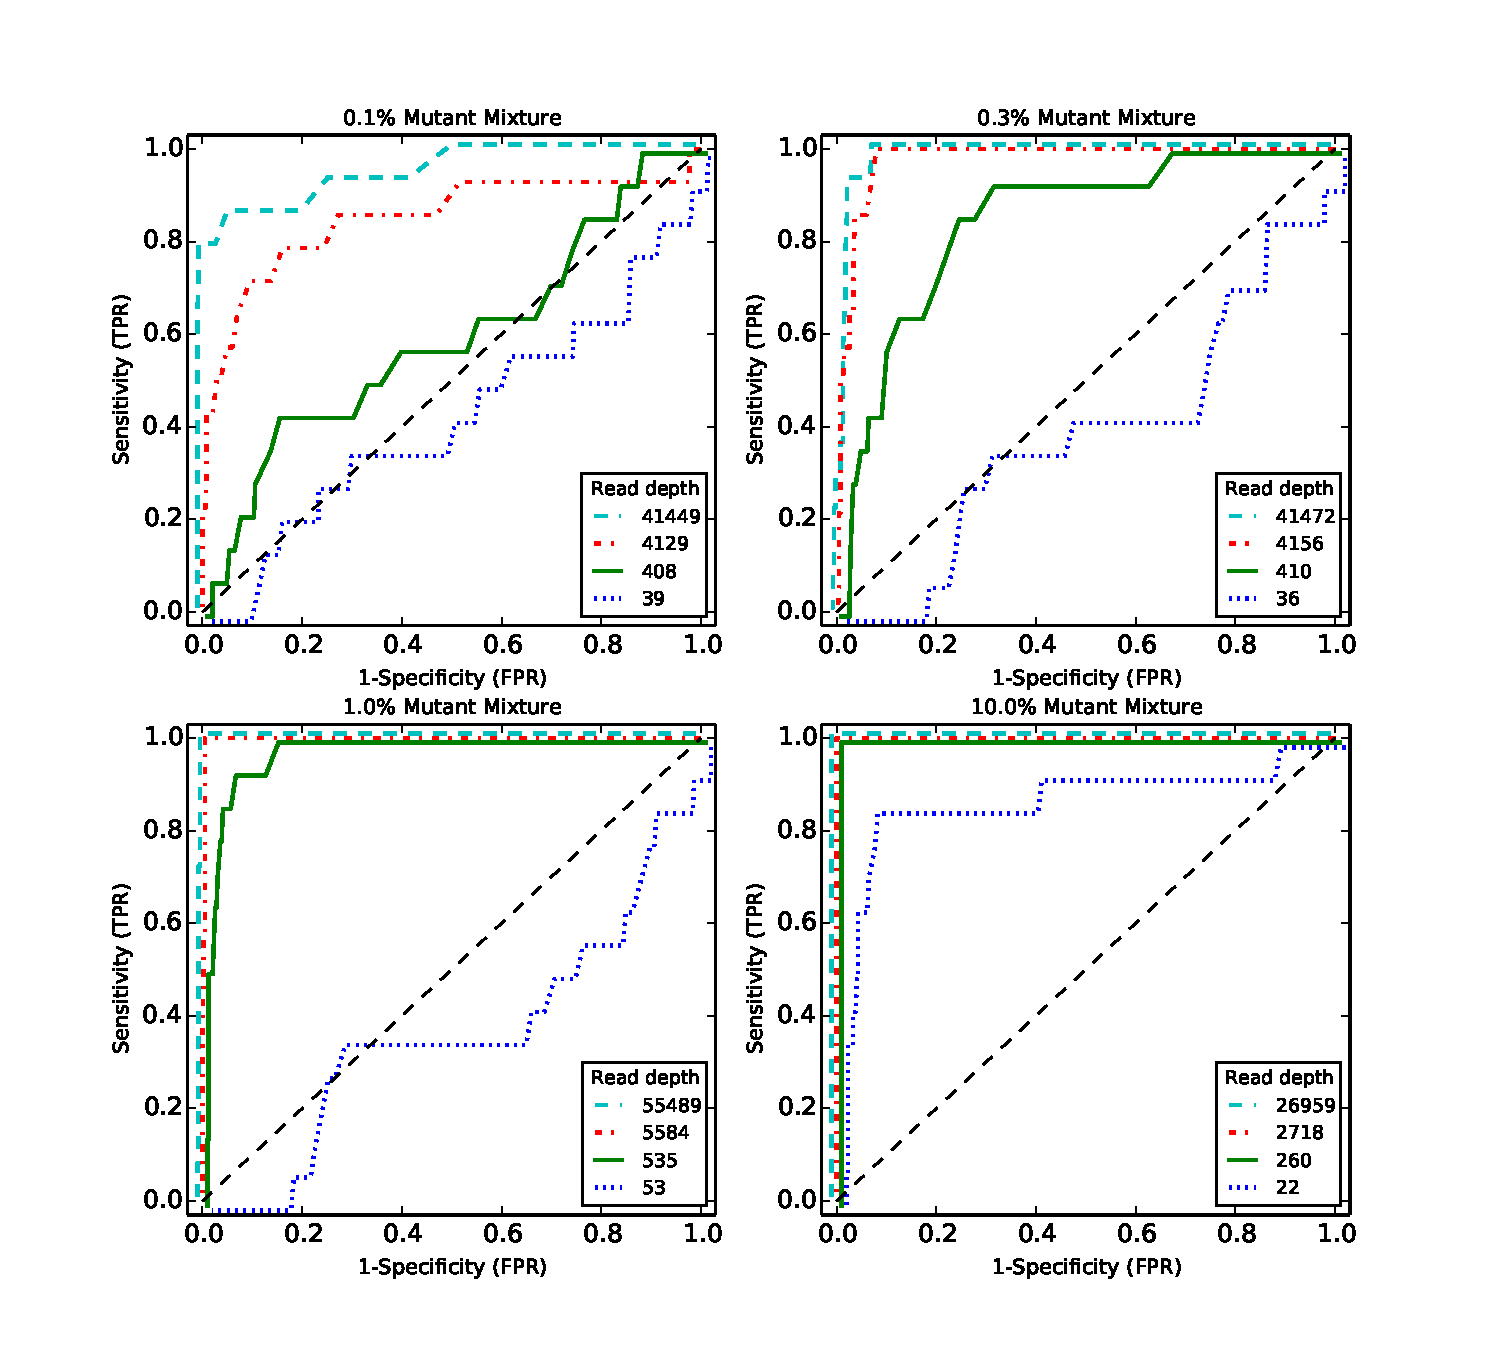
\includegraphics[width=120mm]{pdf_figs/ROC_without_chi2.pdf}
\caption{ROC curve varying read depth showing detection performance.}
\label{fig:ROC}
\end{center}
\end{figure}
% from folder '2013-11-24_six_replicates_Compute_ROC_Synthetic_Qsd_0_1'

Figure~\ref{fig:MAF} shows the posterior mean and 95\% credible intervals for $\mu_j$ for called variant positions with $\bar{n} = 5584$ and MAF = 1.0\%. All of the called positions show a clear difference between the case and control error rates. The posterior mean estimates are all shrunken towards the global error rate parameter $\mu_0 = 0.0023$ due to the hierarchical structure of the model.

\begin{figure}[h]
\begin{center}
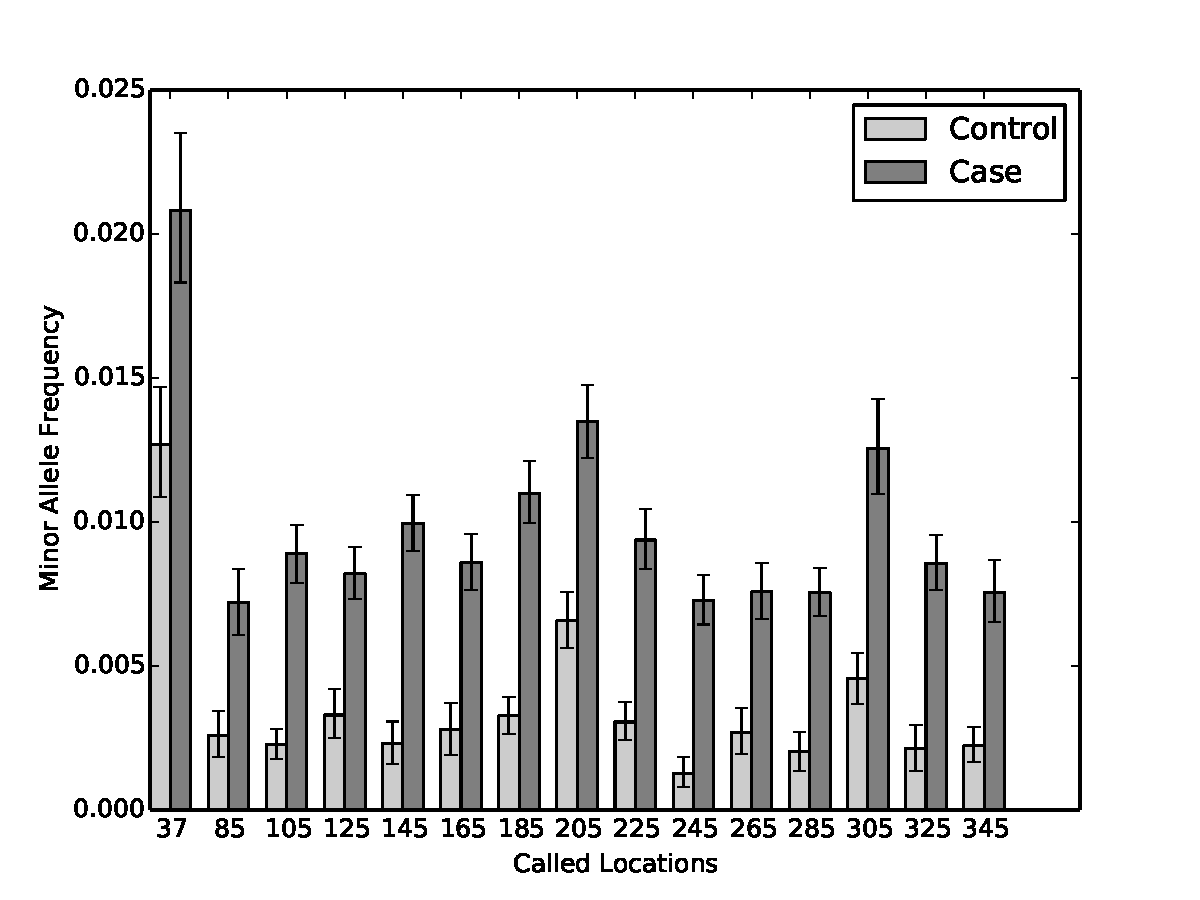
\includegraphics[width=120mm]{pdf_figs/Synthetic_Mubarplot_MAF1_0_Depth5584.pdf}
\caption{Estimated minor allele fraction for called variants in 1.0\% dilution.}
\label{fig:MAF}
\end{center}
\end{figure}
% from folder '2013-11-15_synthetic_mu_barplot_optimalT', dilution rate is 0.1, downsampling rate is 0.01. 


\subsection{Empirical performance compared with other algorithms}\label{sec:comparison}

We compare the empirical performance of RVD2 to other variant calling algorithms using the synthetic DNA data sets using the false discovery rate as well as sensitivity/specificity. In a research applications, the false discovery rate is a more relevant performance metrics because the aim is generally to identify interesting variants. The sensitivity/specificity metric is more relevant in clinical applications where one is more interested in calling all of the true variants and none of the true negatives.

[DISCUSS \citet{Stead:2013fu}] 

\subsubsection*{Sensitivity/Specificity Comparison}

\begin{figure}[h]
\begin{center}
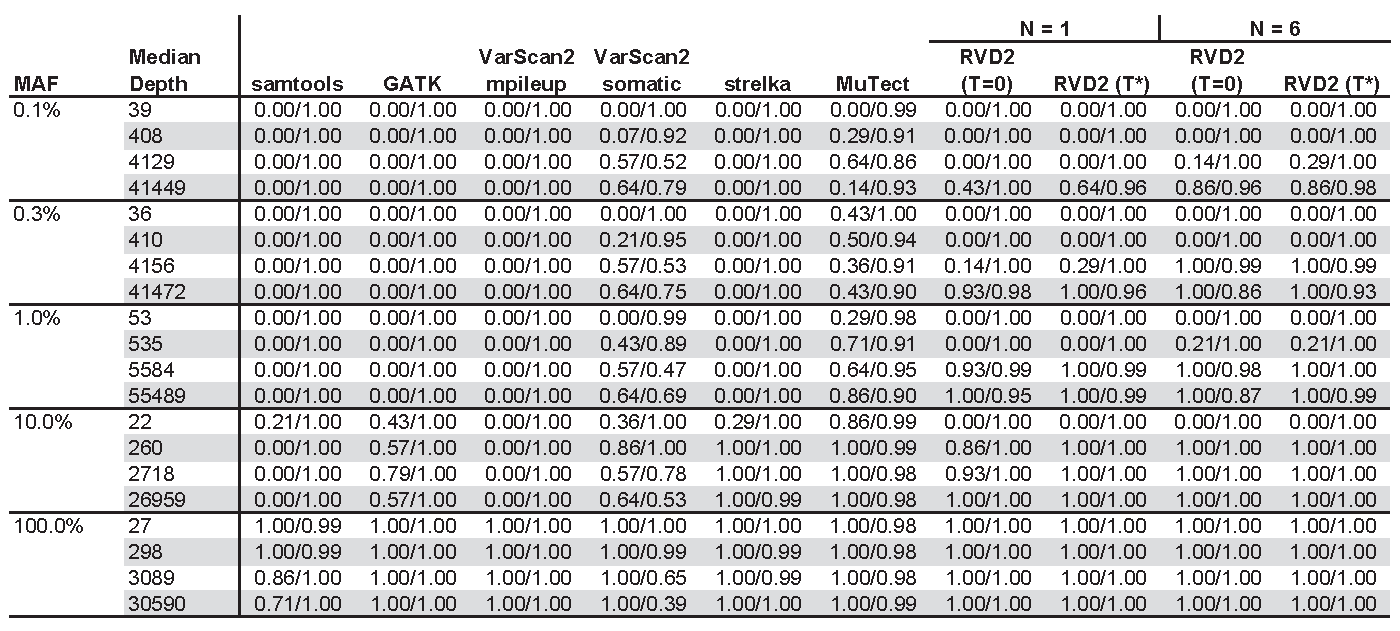
\includegraphics[width=160mm]{pdf_figs/comparison_table_ss.pdf}
\caption{Sensitivity/Specificity comparison of RVD2 with other variant calling algorithms.}
\label{tbl:comparison_ss}
\end{center}
\end{figure}
% from folder 'rvd2\results\2013-09-19_operating_characteristics'
% rvd2 data are from folder '2013-11-12_one_replicate_optT_with_chi','2013-11-12_one_replicate_T_zero_with_chi2','2013-11-15_six_replicates_optT_with_chi2','2013-11-15_six_replicates_T_zero_with_chi2'

Figure~\ref{tbl:comparison_ss} shows that samtools, GATK and VarScan2-mpileup all have similar performance. They call the 100\% MAF experiment well even at low depth, but are unable to identify true variants in mixed samples with much success. VarScan2-somatic is able to call more mixed samples. However, as the read depth increases the specificity degrades. Strelka is able to call 10\% MAF variants with good performance, but is limited at 1\% MAF and below. muTect has good performance across a wide range of MAF levels. But even at the highest depth only has around 0.5 sensitivity for low MAF levels.

The sensitivity for RVD2 with $\tau=0$ is low for low read depths and MAF levels and $N=1$ case and control sample. The sensitivity increases considerably with read depth at a slight expense to specificity. With $\tau^*$ the performance is much better with high sensitivity and specificity across a wide range of read depths and MAFs. However, in practice one may not know the optimal $\tau^*$ a-priori. With $N=6$ replicates, the sensitivity increases considerably for low MAF variants with a slight degradation in specificity due to false positives. When the median read depth is at least $10\times$ the MAF, RVD2 has higher specificity than all of the other algorithms tested and has a lower sensitivity in only three cases. The Matthews correlation coefficient (MCC) indicates that RVD2($\tau=0, N=1$) is more accurate than the other algorithms when the median read depth is at least $10\times$ the MAF (see supplementary table SX).

\subsubsection*{False Discovery Rate Comparison}
Figure~\ref{tbl:comparison_fdr} shows the false discovery rate for RVD2 compared to samtools, GATK, varscan, strelka and muTect. Blank cells indicate no positive calls were made.

Samtools performs well on 100\% MAF sample and performance improves for read depths 3089 and 30590. GATK performs well on both the 10\% and 100\% variants, but makes a false positive call at the 100\% MAF level for all read depth levels. VarScan2-pileup performs perfectly for all but the lowest depth for the 100\% MAF.

\begin{figure}[h]
\begin{center}
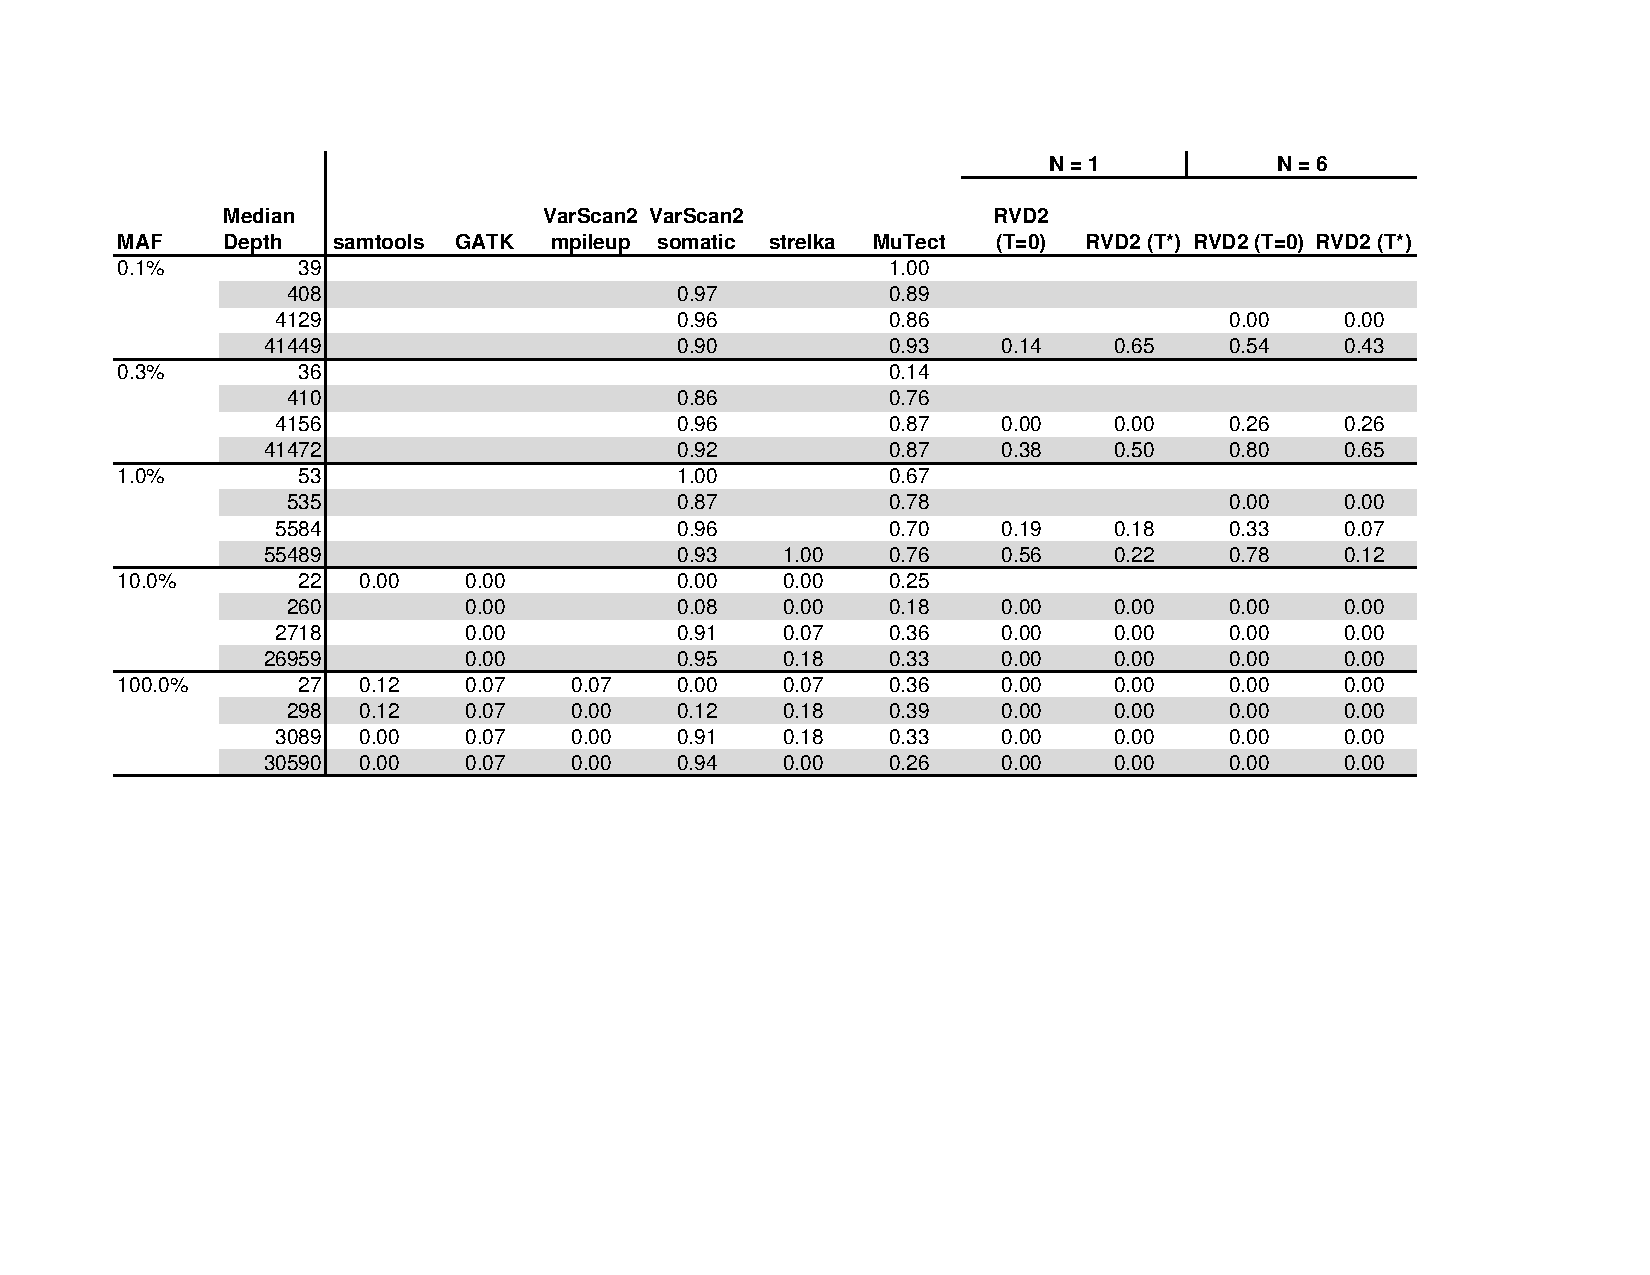
\includegraphics[width=160mm]{pdf_figs/comparison_table_fdr.pdf}
\caption{False discovery rate comparison of RVD2 with other variant calling algorithms. Blank cells indicate no locations were called variant.}
\label{tbl:comparison_fdr}
\end{center}
\end{figure}
% from folder 'rvd2\results\2013-09-19_operating_characteristics'

VarScan2-somatic is able to make calls for all but the lowest MAF and coverage level. However, the FDR is high due to many false positives. Interestingly, at a MAF of 100\% the FDR is zero for lowest read depth and 1.00 for the highest read depth. Strelka has a better FDR than the samtools, GATK or Varscan2-somatic algorithms for almost all read depths at the 10\% and 100\% MAF. However, it does not call any variants at or below 1\% MAF.  MuTect has the best FDR performance of the other algorithms we tested over a wide range of MAF and depths. But the FDR level is relatively high at around 0.7 for 0.1\% -- 1\% MAF and 0.3 for 10\%-100\% MAF.
 
RVD2 has a lower FDR than other algorithms when the read depth is greater than $10\times$ the MAF with $N=1$ and $\tau$ set to the default value of zero or to the optimal value. The FDR is higher when $N=6$ because the variance of the control error rate distribution $P(\mu_j^{\text{control}} | r^{\text{control}})$ is smaller. The smaller variance yields improvements in sensitivity at the expense of more false positives. Since the FDR only considers positive calls, the performance degrades.


\subsection{HCC1187 primary ductal carcinoma sample}\label{sec:brca}

RVD2 identified five variants in the 44kbp PAXIP1 gene from chr7:XXX to chr7:XXX. Of the five called variants, three were homozygous germline variants and two were heterozygous germline variants. The two heterozygous variants had a loss-of-heterozygosity in the tumor sample. 

Figure~\ref{fig:brca_MAF} shows the estimated minor allele frequencies for the normal and tumor samples at the called locations. Positions chr7:154743899C$>$T, chr7:154753635T$>$C and chr7:154780960C$>$T are germline homozygous mutations. Positions chr7:154754371 and chr7:154758813 are called heterozygous in the normal sample. In the tumor cells we identified all five mutations chr7:154743899C$>$T, chr7:154753635T$>$C, chr7:154754371T$>$C, chr7:154758813G$>$A, and chr7:154780960C$>$T. Positions chr7:154754371T$>$C and chr7:154758813G$>$A then loss-of-heterozygosity events.

%According to dbSNPv138 chr7:154743899 is rs1239326, chr7:154753635 is rs1239324, chr7:154754371 is rs71534174, chr7:154758813 is rs35505514, and chr7:154780960 is rs4398858.
%TODO: place these rs labels beneath the position labels on the x-axis of the figure. Remove the above sentence and add. 
%Some of these mutations are also found to be common population SNPs according to dbSNPv138. The corresponding rs identities are shown in the figure.


\begin{figure}[h]
\begin{center}
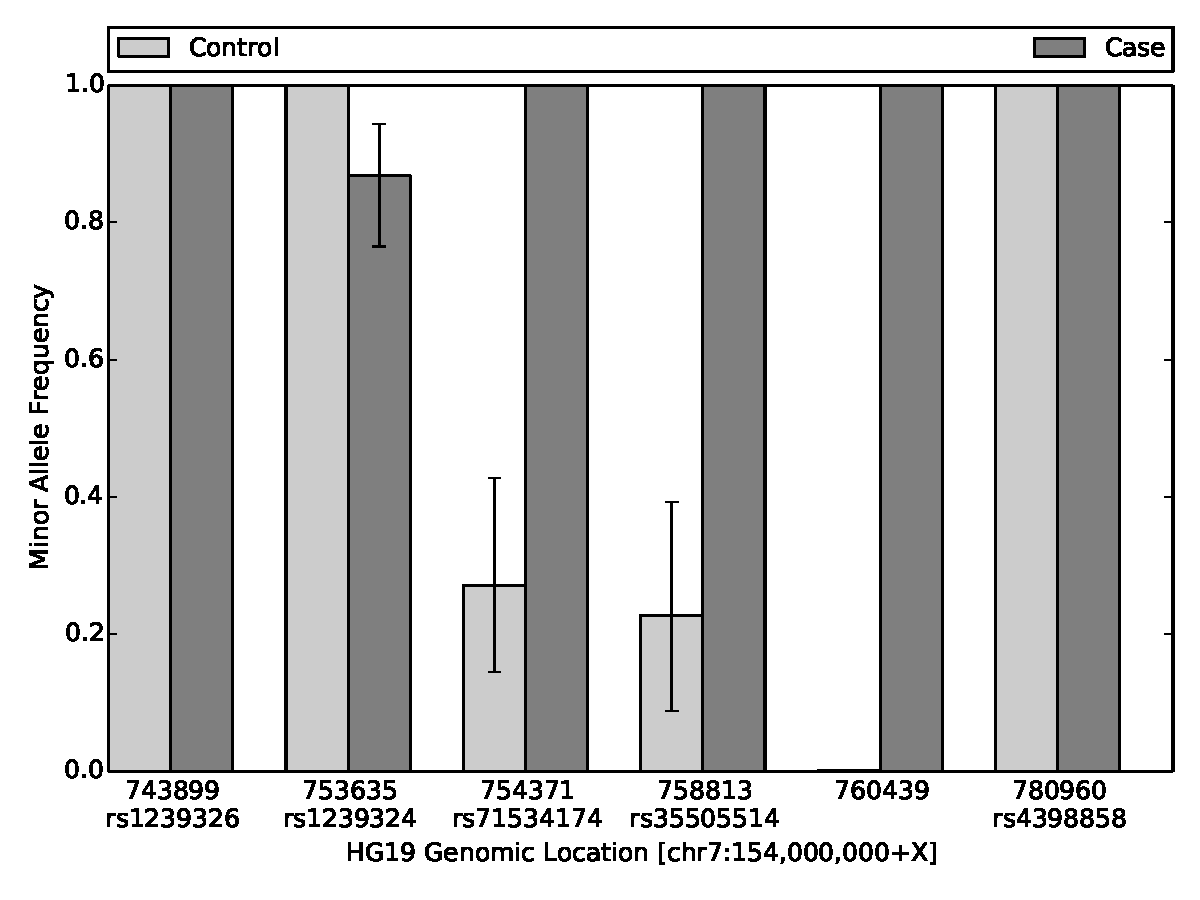
\includegraphics[width=120mm]{pdf_figs/HCC1187_MuBarPlot.pdf}
\caption{Estimated minor allele fraction for called variants in PAXIP1 gene.}
\label{fig:brca_MAF}
\end{center}
\end{figure}
%('rvd2\results\2013-11-21_HCC1187_PAXIP1_mu_barplot_T0')

The original research describing this sample used Strelka to identify mutations in the same sample. They identified chr7:154760439 as variant, but did not call the other four variants. In particular strelka missed the two LOH events.

\section{Discussion}

We describe here a novel algorithm for model estimation and hypothesis testing for identifying single-nucleotide variants in heterogeneous samples using next-generation sequencing data. Our algorithm has a higher sensitivity and specificity than many other approaches for a range of read depths.

Our inference algorithm uses Gibbs sampling and Metropolis-Hastings sampling to estimate the empirical Bayes statistical model. This sampling procedure provides a guarantee to identify the global optimal parameter settings in the long run. However, it may require many samples to achieve that guarantee causing the algorithm to be slower than other deterministic approaches. We opted for this balance of speed and accuracy because computational time is often not limiting and the loss of a false positive or false negative greatly outweighs the cost of more computation.

We have focused on the statistical model and hypothesis test in this study and our results do not include any pre-filtration of erroneous reads or post-filtration of mutation calls beyond a simple quality score threshold. Incorporation of such data-cleaning steps will likely improve the accuracy of the algorithm.

Our approach does not address identification of indels, structural variants or copy number variants. Those mutations typically require specific data analysis models and tests that are different than those for single-nucleotide variants. Furthermore, analysis of RNA-seq data or other data generated on the NGS platform may require different models that are more appropriately tuned to the particular noise feature of that data.

\appendix

%%%%%%%%%%%%%%%%%%%
% Appendix A: Parameter Initialization
%%%%%%%%%%%%%%%%%%%
\section{Parameter Initialization}\label{sec:appendix_mom}
Since $r_{ji} \thicksim \text{Binomial}(n_{ji}, \theta_{ji})$, the first population moment is  $E[r_{ji}] = \theta_{ji} n_{ji}$ and the first sample moment is simply $m_1 = r_{ji}$. Therefore the MoM estimator is 
\begin{equation}
	\tilde{\theta}_{ji} = \frac{r_{ji}} {n_{ji}}
\end{equation}

We take the MoM estimate, $\tilde{\theta}_{ji}$, as data for the next conditional distribution in the hierarchical model. The distribution is $\theta_{ji} \thicksim \text{Beta}(\mu_jM_j, (1-\mu_j)M_j)$. The first and second population moments are
\begin{eqnarray}
	E[\theta_{ji}] =& \mu_j,\\
	\text{Var}[\theta_{ji}] =& \frac{\mu_j(1-\mu_j)} { M_j + 1 }.
\end{eqnarray}
The first and second sample moments are $m_1 = \frac{1}{N}\sum_{i=1}^N \theta_{ji}$ and $m_2 = \frac{1}{N}\sum_{i=1}^N \theta_{ji}^2$. Setting the population moments equal to the sample moments and solving for $\mu_j$ and $M_j$ gives
\begin{eqnarray}
	\tilde{\mu}_j =& \frac{1}{N} \sum_{i=1}^N \theta_{ji}, \\
	\tilde{M_j} =& \frac{ \tilde{\mu}_j (1 - \tilde{\mu}_j ) } { \frac{1}{N} \sum_{i=1}^N \theta_{ji}^2 } -1.
\end{eqnarray}

Following the same procedure for the parameters of $\mu_j \thicksim \text{Beta}(\mu_0, M_0)$ gives the following MoM estimates
\begin{eqnarray}
	\tilde{\mu}_0 =& \frac{1}{J} \sum_{j=1}^J \mu_j \\
	\tilde{M}_0 =& \frac{ \tilde{\mu}_0 (1 - \tilde{\mu}_0 ) } {\frac{1}{J} \sum_{j=1}^J \mu_j^2 } -1.
\end{eqnarray}

%%%%%%%%%%%%%%%%%%%
% Appendix B: Comparison Statistics
%%%%%%%%%%%%%%%%%%%
\section{Algorithm Comparison Statistics}\label{sec:app_comparison}


\begin{figure}[h]
\begin{center}
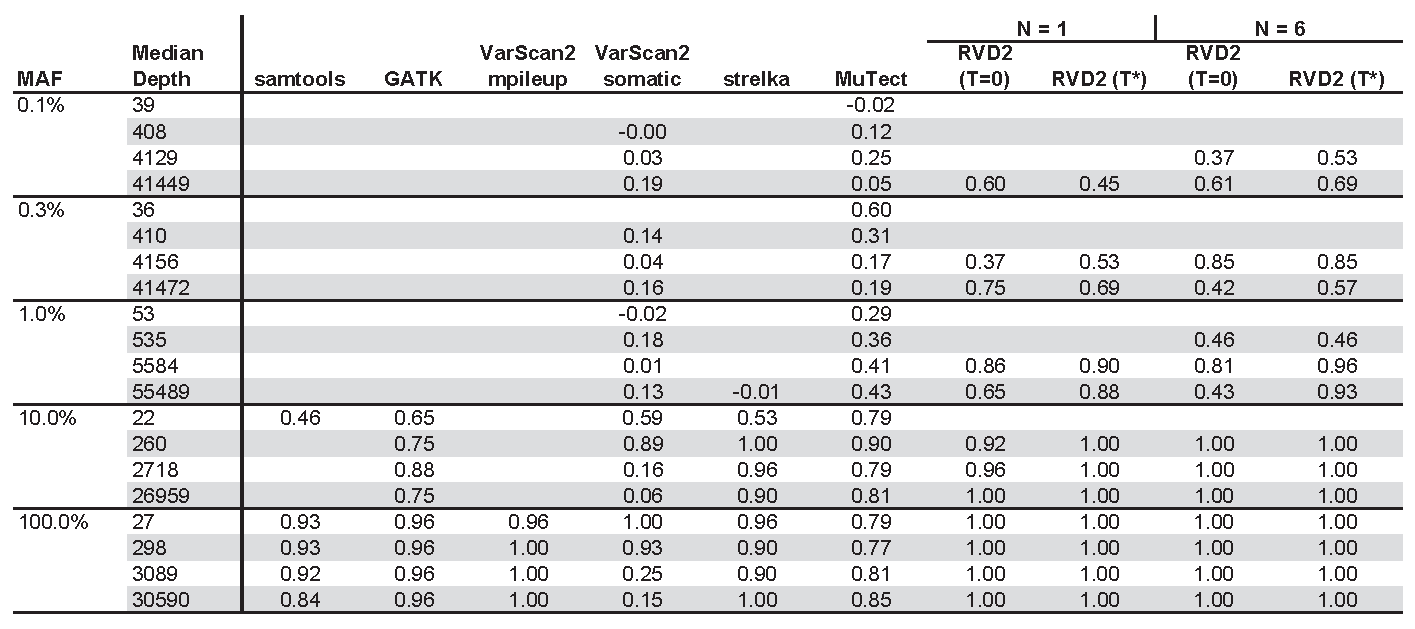
\includegraphics[width=140mm]{pdf_figs/comparison_table_mcc.pdf}
\caption{Matthews correlation coefficient (MCC) comparison with other variant calling algorithms.}
\label{fig:comparison_mcc}
\end{center}
\end{figure}
% from folder 'rvd2\results\2013-09-19_operating_characteristics'



%%%%%%%%%%%%%%%%%
% Appendix C: Data Set Statistics
%%%%%%%%%%%%%%%%%
\section{RVD2 Estimated Parameters}\label{sec:synthetic_estimate}
The RVD2 algorithm provides estimates of model parameters and latent variables given the data. We show several of these parameters in Figure~\ref{fig:depthM}. 

The left column of Figure~\ref{fig:depthM} shows the read depth for each of the six bam files (three replicates each with two read pairs) for each data set. Because the DNA was not sheared and ligated prior to sequencing, the read depth drops to zero at the boundaries. For the 100\% mutant data set, the read depth drops at the mutant locations. This is due to the parameters imposed at the alignment stage. The reads are 36bp long and we required no more than 2 mismatches. Therefore, reads that overlapped two mutations (spaced 20bp apart by design) and included one additional mutation would not align.

\begin{figure}[htbp]
\begin{center}
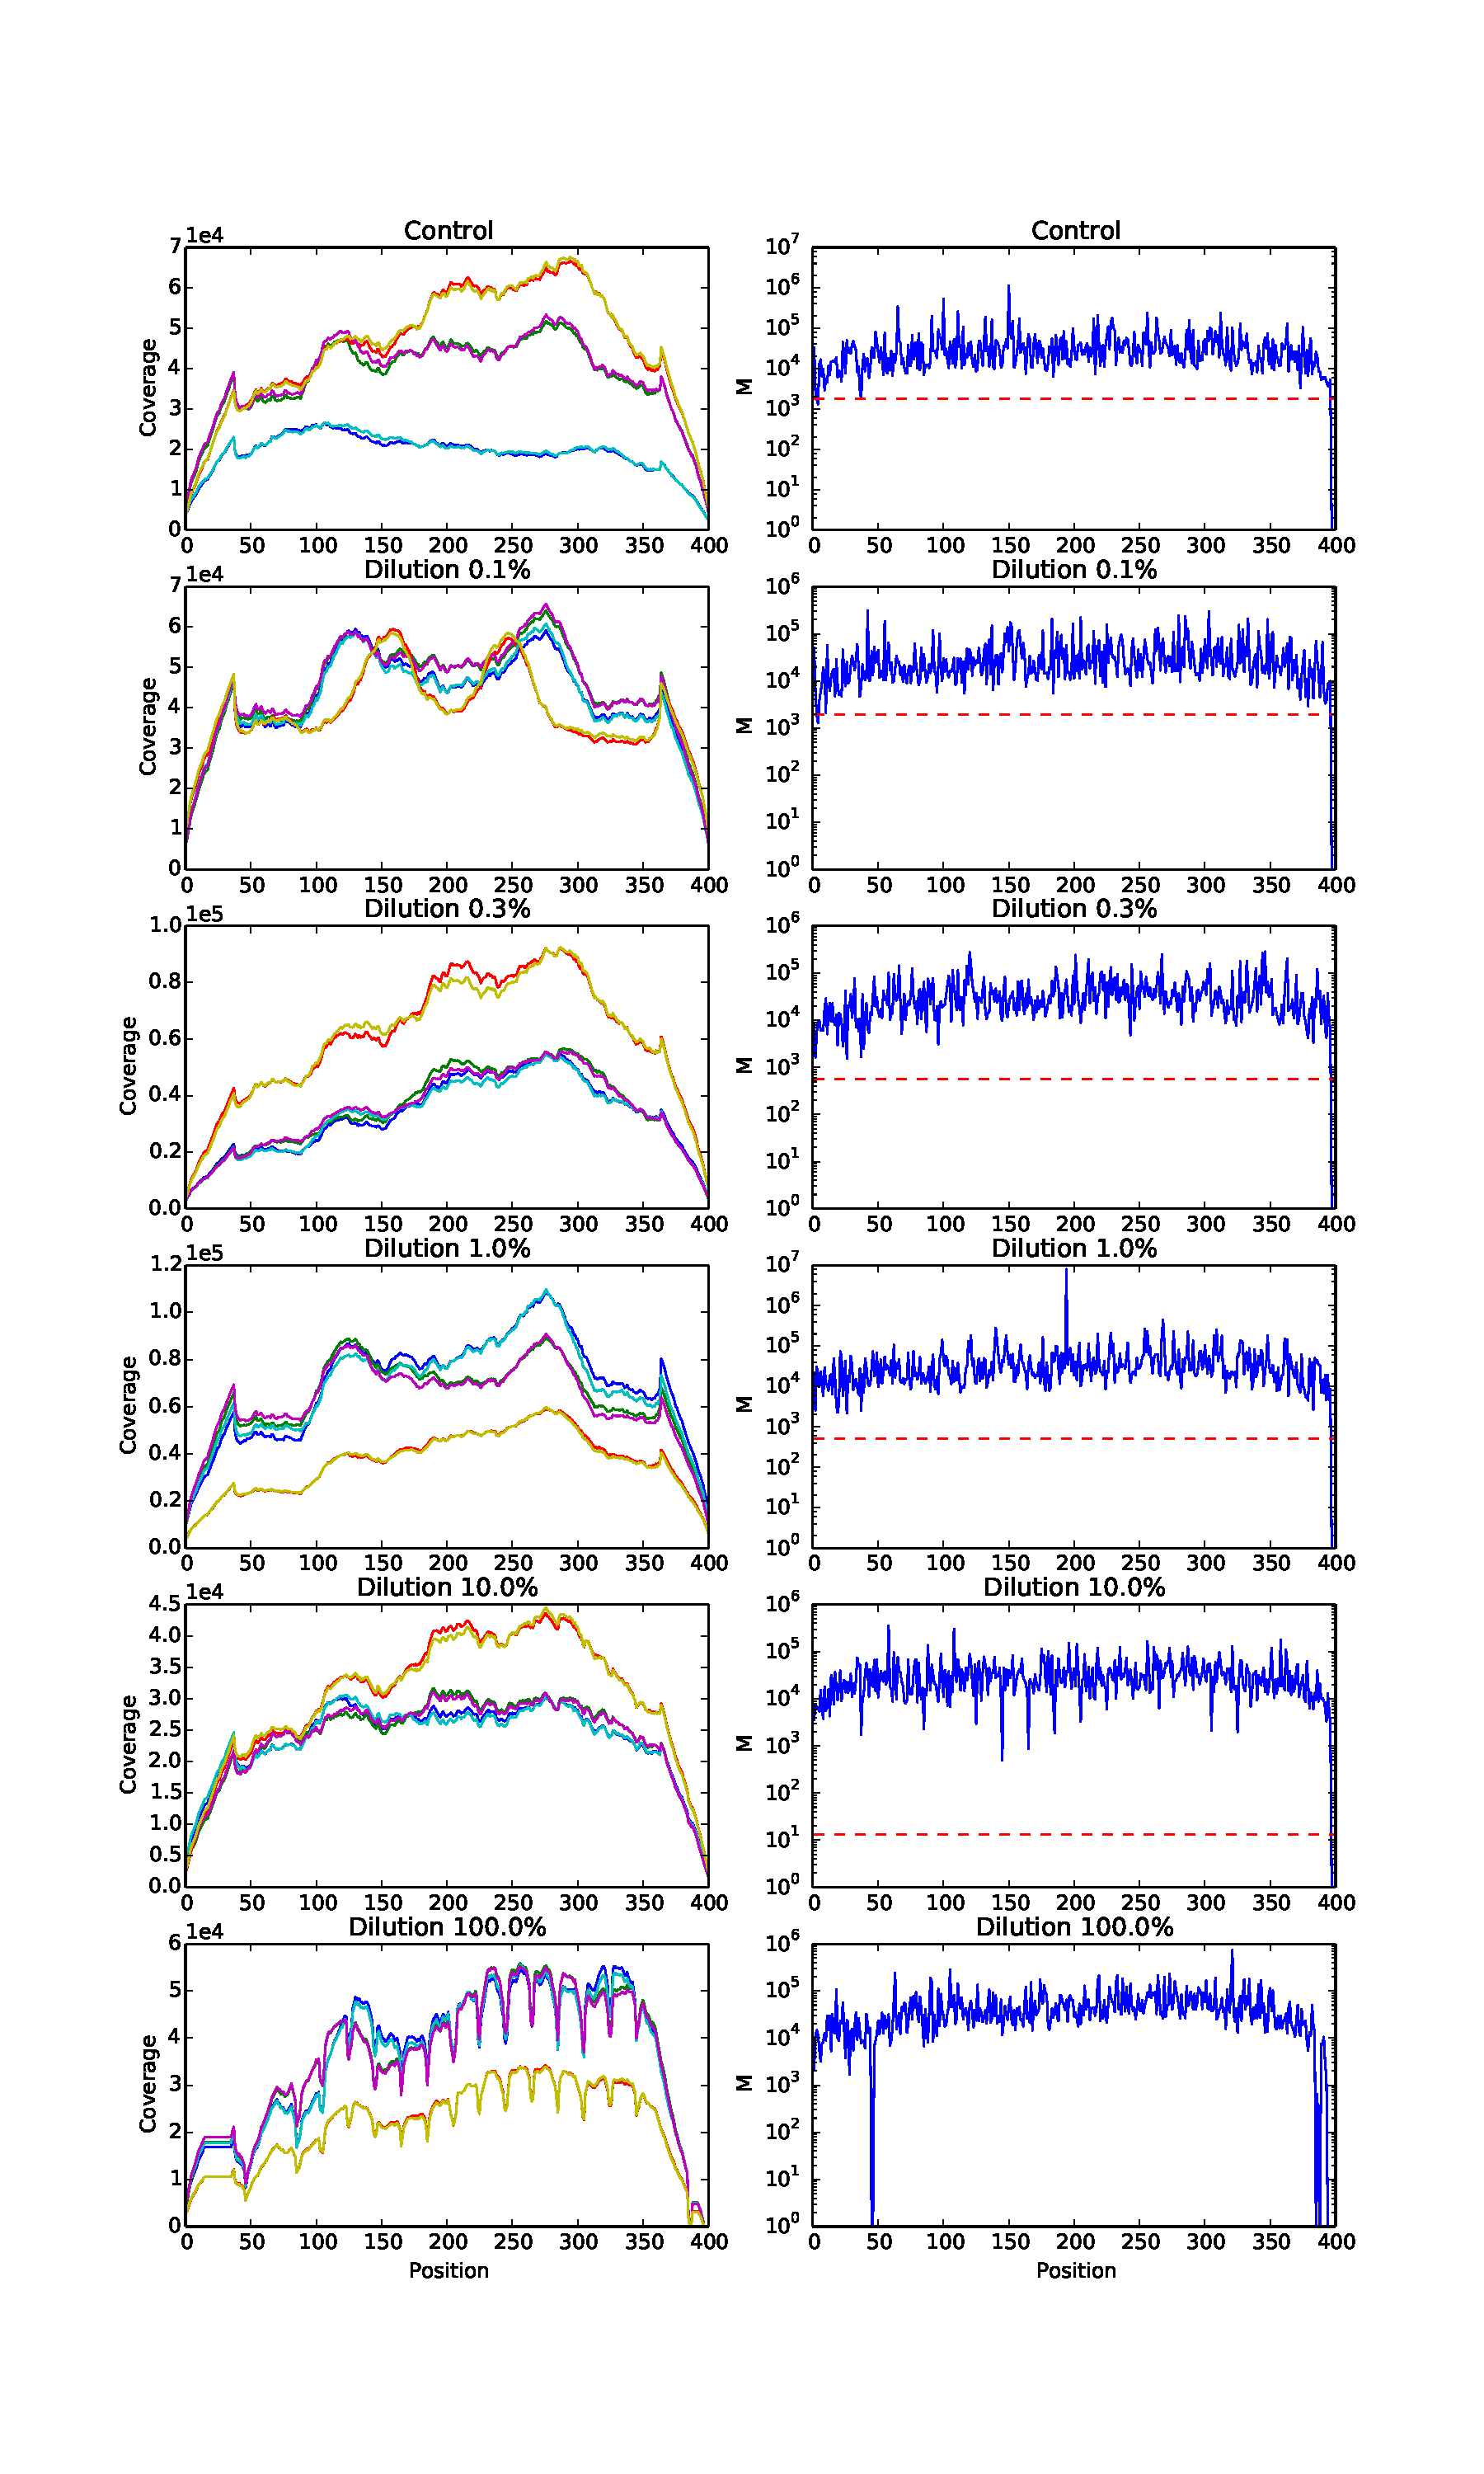
\includegraphics[width=120mm]{pdf_figs/depthM.pdf}
\caption{Key parameters for RVD2 model for synthetic DNA data sets.}
\label{fig:depthM}
\end{center}
\end{figure}

% from folder '22013-11-15_depthM_plot_avg10', dilution rate is 0.1.

The right column of Figure~\ref{fig:depthM} shows the parameter estimates $\hat{M}_j$ and $\hat{M}_0$ for each data set. $M_j$ measures the variance between replicates at location $j$. There is little variability across positions indicating that the replication variance does not change greatly across position. Furthermore, we see that $M_j$ does not change with read depth (except where the depth goes to zero) indicating that $M_j$ because $M_j$ is capturing a different process than the read depth. 

The error rate across positions is captured by the $M_0$ parameter shown as a horizontal dotted line in the plots in the right column. We see that the variation between replicates is smaller than the variation between location. $M_j$ and $M_0$ are precision parameters, they are inversely proportional to the variance. Where $M_j$ is greater than $M_0$ the precision between replicates is higher than the precision across positions.


%%%%%%%%%%%%%%%%%
% Appendix D: Parameter Settings for Variant Calling Algorithms
%%%%%%%%%%%%%%%%%
\section{Parameter settings for other variant calling algorithms}

\paragraph{\textbf{Samtools}}We used samtools/bcftools (v0.1.19) for variant calling. mpileup was the function to call variants and bcftools was used to save the result in standard Variant Call Format (VCF) files. In mpileup, we set the -d option sufficiently high at $10^6$ to avoid coverage cap.  mpileup was able to accept multiple replicates at one time so six bam files from each replicate group were fed into mpileup for variant calling. Read depth for each sample was kept with -D enabled, and -u was turned on to make sure the output bcf files uncompressed. 

\paragraph{\textbf{GATK}}
UnifiedGenotyper is the function we used in GATK (v2.1-8) to detect mutations.We followed the general GATK recomended workflow to detect variants. Due to some format  incompatibility, we applied Picard to format read group and GATK for realignment as preprocessing. When calling variants using UnifiedGenotyper, -ploid (Number of samples in each pool $\times$ Sample Ploidy) was set at 1 because our synthetic data is haploid; we change the default setting for -dcov (default max coverage cutoff of $250\times$ ) to $10^6$ to avoid downsamplig so that the coverage was comparable to other approaches. All other parameters were set at default. Six replicates was passed to GATK for variant calling.

\paragraph{\textbf{VarScan2-mpileup}}
VarScan2 (v2.3.4) mpileup2snp is a SNP calling program which takes multi-samples from samtools mpileup pipeline. We set -d at $10^6$ and enabled -50 for same concern previously stated. In afterwards mpileup2snp function, --min-var-freq, the only non-default parameter, was set low enough at $10^{-5}$ because the variant frequency can be as low as $10^{-3}$. Six replicates were all introduced for variant calling.

\paragraph{\textbf{VarScan2-somatic}}
We tested VarScan2-somatic on our six replicates synthetic data set as well. Considering that RVD2 doesn't call somatic status, we combined all the positions VarScan2-somatic called regardless the somatic status (Germline/LOH/Somatic/Unknown). --normal-purity was set at 1.00, while --tumor-purity was set as the dilution rate. --min-var-freq was set at $10^{-5}$.

\paragraph{\textbf{Strelka}}
Configuration and Analysis for Strelka is standard so we just installed the program and ran it on our data set. One thing to note is that since Strelka can not accept relicate data, we used a single replicate with a read depth that most closely matched the overall median depth of the replicates.

\paragraph{\textbf{muTect}}
Similar to Strelka, we ran muTect with standard settings and only passed one replicate of synthetic data.

GATK, samtools and VarScan2-mpileup are optimized to call genotypes on pure samples. Therefore, we expect those algorithms to perform well on the 100\% dilution (pure mutant) sample and poorly on heterogeneous samples. \citet{Stead:2013fu} showed that varscan-somatic outperformed Strelka had performance on-par with muTect in detecting a 5\% MAF for read depths between 100 and 1000. We find its performance on much lower MAF variants and across a wider range of coverage depths. Varscan2-somatic, strelka and muTect do not accept replicate data for the ``normal" or ``tumor" bam files so we used a single bam file from each replicate group with a read depth that most closely matched the overall median depth of the replicates.

\bibliographystyle{apalike}
\bibliography{bioinfo}
\end{document}  
